\newpage
\section{Проектирование}
Выше были выделены основные компоненты системы и разграничены функции и
ответственность между ними. Теперь необходимо определиться с конкретной
реализацией выбранных компонентов и со схемой взаимодействия между ними. 
Общая архитектура системы представлена на рисунке
\ref{ris:general_architecture}. Нижу будут рассмотрены основные компоненты
и описаны их назначения.

\begin{figure}[h]
\center{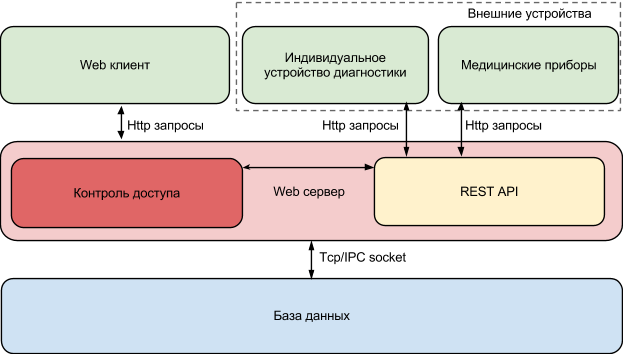
\includegraphics[width=1\linewidth]{general_architecture.eps}}
\caption{Общая архитектура системы.}
\label{ris:general_architecture}
\end{figure}

\subsection{Web клиент}
Клиент разделяет функции подсистемы ввода данных и подсистемы доступа к данным.
Основной задачей клиента является предоставление доступа к системе пользователям
с помощью веб-браузера или другого программного обеспечения способного работать
с протоколом HTTP. С точки зрения требования доступности, реализация в виде web
клиента наиболее оптимальна, так как веб-браузеры есть на всех современных
платформах и устройствах.

\subsection{Web сервер}
Основной задачей Web сервера является - организация взаимодействия между
различными клиентами и системой хранения данных. Также в рамках Web сервера
будут реализованы:
\begin{enumerate}
  \item бизнес-логика системы;
  \item контроль доступа к системе;
  \item подсистема унифицированного доступа к системе хранения данных;
  \item подсистема анализа данных;
  \item REST API для унифицированного взаимодействия с внешними источниками и
потребителями данных.
\end{enumerate}

\subsection{REST API}
Основной задачей является предоставление публичного интерфейса для ввода данных
с внешних источников.

\subsection{База данных}
Достаточно долгое время основным типом системы хранения данных была SQL база
данных. Однако в последние годы получает распространение NoSQL системы хранения.
Данные подходы к организации источника данных преследуют одну цель - обеспечить
долговременное, надежное хранение структурированных данных. Каждый подход имеет
свои преимущества и недостатки.
Для того чтобы определится какого типа будет система хранения данных необходимо
сформировать требования к системе, а затем на основании требований выбрать
наиболее подходящий тип системы.

\subsubsection{Требования к системе хранения данных}
Надежность - очень широкое понятие в терминах баз данных. Рассмотрим основные
составляющие надежной системы хранения.
\subparagraph{Обеспечение целостности данных.}
SQL системы изначально проектировались чтобы соответствовать основным принципам
ACID и как следствие предоставляют возможность хранить данные в нормализованном
виде, явно определяя связи между элементами базы даных. Однако такой подход
несет дополнительную нагрузку на базу данных, т.к. необходимо констролировать
целостность данных а базе.
NoSQL решения изначально проектировались как полная альтернатива SQL решениям.
Они позволяют хранить данные в максимально денормализованном виде. При таком
подходе вся ответственность за целостность даных возлагается целиком на
разработчиков.
\subparagraph{Масштабируемость.} 
При росте числа пользователей базы данных возникает проблема обработки большого
числа запросов к базе данных. Данную проблему можно решить за счет
горизонтальной или вертикальной масштабируемости ситемы.

При вертикальной масштабируемости предлагается обновлять конфигурацию сервера на
более современную для повышения производительности. При таком подходе очевидно
что общая производительность ситемы, если не брать в счет програмную
составляющую, ограничивается только прогресом в области производства аппаратного
обеспечения. Как правило местом преткновения становится скорость операций i/o на
жестком диске. Также стоит учитывать что цены на новинки всегда завышены и
нецелесообразно будет платить достаточно крупные суммы за повышение
производительности на несколько процентов.

При горизонтальном масштабировании предлагается распределять нагрузку на
несколько серверов баз данных. При таком подходе не нужно покупать новое
дорогостоящее оборудование, производительность не упирается в скорость i/o
операций на жестком диске, а производительность системы повышается
прямопропорционально числу серверов. Достаточно обеспечить необходимое
количество серверов чтобы балансировать нагрузку между ними.
На самом деле на этом вопрос масштабируемости не ограничивается, т.к. необходимо
учитывать еще один важный фактор - размер базы данных. Некоторые современные
базы данных поддерживают механизм партицирования. Данный механизм позволяет
разбивать таблицу на несколько частей. В результате чего возможно хранить данные
на разных носителях. Данный механиз повышает скорость доступа к данным за счет
того что выборка манипуляции с даными происходят не в контексте всей таблицы а в
контексте конкретной части таблицы. Не стоит забывать и о выборе файловой
системы под файлы базы данных и драйвера который будет управлять распределением
данных в файловой системе.
\subparagraph{Быстродействие.} 

Скорость работы подсистемы хранения данных непосредственно влияет на
продолжительность приема. Важно чтобы доступ к данным был максимально быстрым.

SQL решение накладывает некоторые ограничения. Прежде всего это индексы и
транзакции, которые могут заметно снизить скорость вставки данных, но без них
может значительно снижаться скорость выбрки данных.

NoSQL решение потенциально не имеет проблем со вставкой данных. Теоретически
вставка данных должна происходить со скоростью равной скорости записи в
оперативную память. Стоит отметить что все современные SQL базы данных
производят первичную запись данных так же в оперативную память.

\subparagraph{Выбор между SQL и NoSQL.}
Выбор между двумя подходами достаточно сложная задача. В рамках выбранной
предметной области система может быть спроектирована как NoSQL так и SQL
подходом. Однако SQL подход обеспечивает большую согласованность данных и более
простую реализацию. Так же немаловажным фактором в пользу SQL подхода является
наличие более развитых средств разработки.


